
\section{Results}

(for rough draft...)

Looks like M6 and M8 are the best meta-refactorings according to ANOVA.
If you peek at MTResults Processing.csv on google docs, M6 has the best refactoring...every OCTAL type should be converted to an OR or preferably a CCC.

M8 has a weak P value, but still ok in one case (0.12) and consistently says that 'aa*' should be written as 'a+'.

Looks like M0, M1, M2, M3 and M9 are very dependent on the regex chosen, so regex-specific refactorings like:
0.1401 \verb!&d([aeiou][aeiou])z'    &d([aeiou]{2})z'!
0.075   \verb![\t\r\f\n ]'    [\s]'!
0.1024  \verb![a-f]([0-9]+)[a-f]' [a-f](\d+)[a-f]'!
0.1271  \verb![\{][\$](\d+[.]\d)[}]'!
\verb!\\\{\\\$(\d+\.\d)\}'!
(from M0,M1,M2,M9 respectively)

have okay P-values and may indicate regex-specific refactorings, but do not indicate an overall trend for that type of refactoring.
Notice that M3 does not even have a strong p-value candidate, but this may be thrown off because of the very confusing regex chosen for CCC:
0.78    0.79
\verb!xyz[_\[\]`\^\\]'!    \verb!xyz[\x5b-\x5f]'!
which has a lot of escape characters, so that the hex group was easier to understand than the CCC.



Meanwhile M4,M5 and M7 have both ambiguous p-values and anova results.  But this is still a finding: that no refactoring is needed between things like:
\verb!(q4fab|ab)'! (\verb!(q4f){0,1}ab)'!
\verb!tri[abcdef]3'!   \verb!tri(a|b|c|d|e|f)3'!
\verb!&(\w+);'!    \verb!&([A-Za-z0-9_]+);'!
(from M4,M5,M7 respectively)

Although one refactoring from M5 might be of slight interest:
0.1196  FALSE   \verb!tri[a-f]3'!  \verb!tri(a|b|c|d|e|f)3'!


\begin{figure*}[tb]
\centering
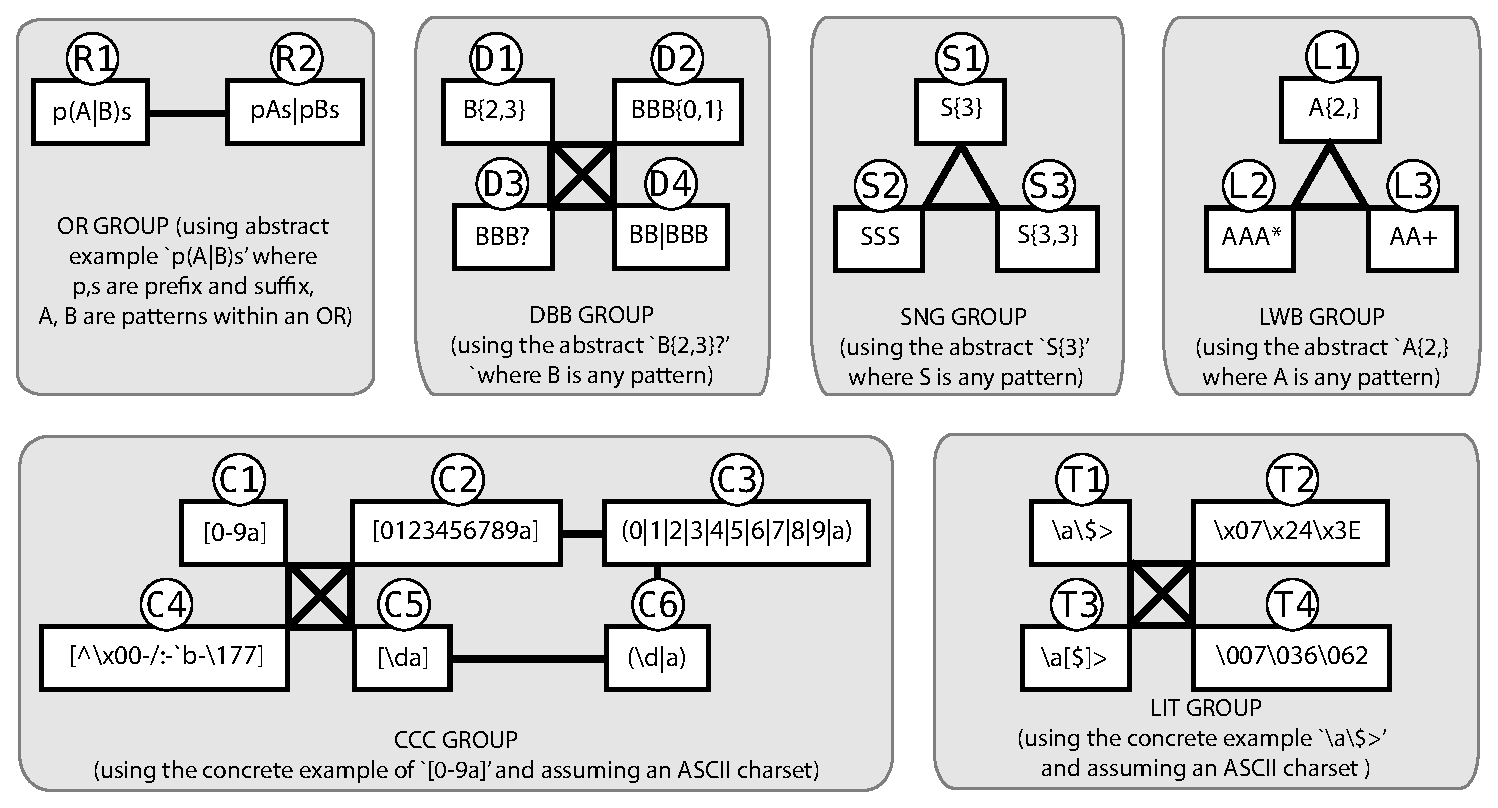
\includegraphics[width=\textwidth]{illustrations/refactoringTree.eps}
\vspace{-12pt}
\caption{Some possible refactorings}
\vspace{-6pt}
\label{fig:refactoringTree}
\end{figure*}

\todoMid{more data from the composition problems}
